%%%%%%%%%%%%%%%%%%%%%%%%%%%%%%%%%%%%%%%%%
% Cleese Assignment (For Students)
% LaTeX Template
% Version 2.0 (27/5/2018)
%
% This template originates from:
% http://www.LaTeXTemplates.com
%
% Author:
% Vel (vel@LaTeXTemplates.com)
%
% License:
% CC BY-NC-SA 3.0 (http://creativecommons.org/licenses/by-nc-sa/3.0/)
% 
%%%%%%%%%%%%%%%%%%%%%%%%%%%%%%%%%%%%%%%%%

%----------------------------------------------------------------------------------------
%	PACKAGES AND OTHER DOCUMENT CONFIGURATIONS
%----------------------------------------------------------------------------------------

\documentclass[11pt]{article}
\usepackage{listings}
\usepackage{float}
\usepackage{color} %red, green, blue, yellow, cyan, magenta, black, white
\definecolor{mygreen}{RGB}{28,172,0} % color values Red, Green, Blue
\definecolor{mylilas}{RGB}{170,55,241}
\usepackage{hyperref}
\usepackage[printwatermark]{xwatermark}
\newwatermark[allpages,color=gray!50,angle=45,scale=2.5,xpos=-5,ypos=-5]{Mohammad Hadi}

%%%%%%%%%%%%%%%%%%%%%%%%%%%%%%%%%%%%%%%%%
% Cleese Assignment
% Structure Specification File
% Version 1.0 (27/5/2018)
%
% This template originates from:
% http://www.LaTeXTemplates.com
%
% Author:
% Vel (vel@LaTeXTemplates.com)
%
% License:
% CC BY-NC-SA 3.0 (http://creativecommons.org/licenses/by-nc-sa/3.0/)
% 
%%%%%%%%%%%%%%%%%%%%%%%%%%%%%%%%%%%%%%%%%

%----------------------------------------------------------------------------------------
%	PACKAGES AND OTHER DOCUMENT CONFIGURATIONS
%----------------------------------------------------------------------------------------

\usepackage{lastpage} % Required to determine the last page number for the footer

\usepackage{graphicx} % Required to insert images

\setlength\parindent{0pt} % Removes all indentation from paragraphs

\usepackage[most]{tcolorbox} % Required for boxes that split across pages

\usepackage{booktabs} % Required for better horizontal rules in tables

\usepackage{listings} % Required for insertion of code

\usepackage{etoolbox} % Required for if statements

%----------------------------------------------------------------------------------------
%	MARGINS
%----------------------------------------------------------------------------------------

\usepackage{geometry} % Required for adjusting page dimensions and margins

\geometry{
	paper=a4paper, % Change to letterpaper for US letter
	top=3cm, % Top margin
	bottom=3cm, % Bottom margin
	left=2.5cm, % Left margin
	right=2.5cm, % Right margin
	headheight=14pt, % Header height
	footskip=1.4cm, % Space from the bottom margin to the baseline of the footer
	headsep=1.2cm, % Space from the top margin to the baseline of the header
	%showframe, % Uncomment to show how the type block is set on the page
}

%----------------------------------------------------------------------------------------
%	FONT
%----------------------------------------------------------------------------------------

\usepackage[utf8]{inputenc} % Required for inputting international characters
\usepackage[T1]{fontenc} % Output font encoding for international characters

\usepackage[sfdefault,light]{roboto} % Use the Roboto font

%----------------------------------------------------------------------------------------
%	HEADERS AND FOOTERS
%----------------------------------------------------------------------------------------

\usepackage{fancyhdr} % Required for customising headers and footers

\pagestyle{fancy} % Enable custom headers and footers

\lhead{\small\assignmentClass\ifdef{\assignmentClassInstructor}{\ (\assignmentClassInstructor):}{}\ \assignmentTitle} % Left header; output the instructor in brackets if one was set
\chead{} % Centre header
\rhead{\small\ifdef{\assignmentAuthorName}{\assignmentAuthorName}{\ifdef{\assignmentDueDate}{Due\ \assignmentDueDate}{}}} % Right header; output the author name if one was set, otherwise the due date if that was set

\lfoot{} % Left footer
\cfoot{\small Page\ \thepage\ of\ \pageref{LastPage}} % Centre footer
\rfoot{} % Right footer

\renewcommand\headrulewidth{0.5pt} % Thickness of the header rule

%----------------------------------------------------------------------------------------
%	MODIFY SECTION STYLES
%----------------------------------------------------------------------------------------

\usepackage{titlesec} % Required for modifying sections

%------------------------------------------------
% Section

\titleformat
{\section} % Section type being modified
[block] % Shape type, can be: hang, block, display, runin, leftmargin, rightmargin, drop, wrap, frame
{\Large\bfseries} % Format of the whole section
{\assignmentQuestionName~\thesection} % Format of the section label
{6pt} % Space between the title and label
{} % Code before the label

\titlespacing{\section}{0pt}{0.5\baselineskip}{0.5\baselineskip} % Spacing around section titles, the order is: left, before and after

%------------------------------------------------
% Subsection

\titleformat
{\subsection} % Section type being modified
[block] % Shape type, can be: hang, block, display, runin, leftmargin, rightmargin, drop, wrap, frame
{\itshape} % Format of the whole section
{(\alph{subsection})} % Format of the section label
{4pt} % Space between the title and label
{} % Code before the label

\titlespacing{\subsection}{0pt}{0.5\baselineskip}{0.5\baselineskip} % Spacing around section titles, the order is: left, before and after

\renewcommand\thesubsection{(\alph{subsection})}

%----------------------------------------------------------------------------------------
%	CUSTOM QUESTION COMMANDS/ENVIRONMENTS
%----------------------------------------------------------------------------------------

% Environment to be used for each question in the assignment
\newenvironment{question}{
	\vspace{0.5\baselineskip} % Whitespace before the question
	\section{} % Blank section title (e.g. just Question 2)
	\lfoot{\small\itshape\assignmentQuestionName~\thesection~continued on next page\ldots} % Set the left footer to state the question continues on the next page, this is reset to nothing if it doesn't (below)
}{
	\lfoot{} % Reset the left footer to nothing if the current question does not continue on the next page
}

%------------------------------------------------

% Environment for subquestions, takes 1 argument - the name of the section
\newenvironment{subquestion}[1]{
	\subsection{#1}
}{
}

%------------------------------------------------

% Command to print a question sentence
\newcommand{\questiontext}[1]{
	\textbf{#1}
	\vspace{0.5\baselineskip} % Whitespace afterwards
}

%------------------------------------------------

% Command to print a box that breaks across pages with the question answer
\newcommand{\answer}[1]{
	\begin{tcolorbox}[breakable, enhanced]
		#1
	\end{tcolorbox}
}

%------------------------------------------------

% Command to print a box that breaks across pages with the space for a student to answer
\newcommand{\answerbox}[1]{
	\begin{tcolorbox}[breakable, enhanced]
		\vphantom{L}\vspace{\numexpr #1-1\relax\baselineskip} % \vphantom{L} to provide a typesetting strut with a height for the line, \numexpr to subtract user input by 1 to make it 0-based as this command is
	\end{tcolorbox}
}

%------------------------------------------------

% Command to print an assignment section title to split an assignment into major parts
\newcommand{\assignmentSection}[1]{
	{
		\centering % Centre the section title
		\vspace{2\baselineskip} % Whitespace before the entire section title
		
		\rule{0.8\textwidth}{0.5pt} % Horizontal rule
		
		\vspace{0.75\baselineskip} % Whitespace before the section title
		{\LARGE \MakeUppercase{#1}} % Section title, forced to be uppercase
		
		\rule{0.8\textwidth}{0.5pt} % Horizontal rule
		
		\vspace{\baselineskip} % Whitespace after the entire section title
	}
}

%----------------------------------------------------------------------------------------
%	TITLE PAGE
%----------------------------------------------------------------------------------------

\author{\textbf{\assignmentAuthorName}} % Set the default title page author field
\date{} % Don't use the default title page date field

\title{
	\thispagestyle{empty} % Suppress headers and footers
	\vspace{0.2\textheight} % Whitespace before the title
	\textbf{\assignmentClass:\ \assignmentTitle}\\[-4pt]
	\ifdef{\assignmentDueDate}{{\small Due\ on\ \assignmentDueDate}\\}{} % If a due date is supplied, output it
	\ifdef{\assignmentClassInstructor}{{\large \textit{\assignmentClassInstructor}}}{} % If an instructor is supplied, output it
	\vspace{0.32\textheight} % Whitespace before the author name
}
 % Include the file specifying the document structure and custom commands

%----------------------------------------------------------------------------------------
%	ASSIGNMENT INFORMATION
%----------------------------------------------------------------------------------------

% Required
\newcommand{\assignmentQuestionName}{Task} % The word to be used as a prefix to question numbers; example alternatives: Problem, Exercise
\newcommand{\assignmentClass}{Communication Systems (Taught by Mohammad Hadi)\\Final Project (Due on DDD.,\ mmm.\ dd,\ yyyy)} % Course (Lecturer)\\Assignment (Due date)
\newcommand{\assignmentTitle}{} % Assignment title or name
\newcommand{\assignmentAuthorName}{ALI BAGHERI\\96101302} % Student name\\Student number
%----------------------------------------------------------------------------------------

\begin{document}

%----------------------------------------------------------------------------------------
%	TITLE PAGE
%----------------------------------------------------------------------------------------

\assignmentSection{Simulation Task}


\begin{question}

\questiontext{Here, we intend to simulate a realtime communication system in MATLAB. Consider the general block diagram of Fig. \ref{fig:model}.}
\begin{figure}[h]
\centering
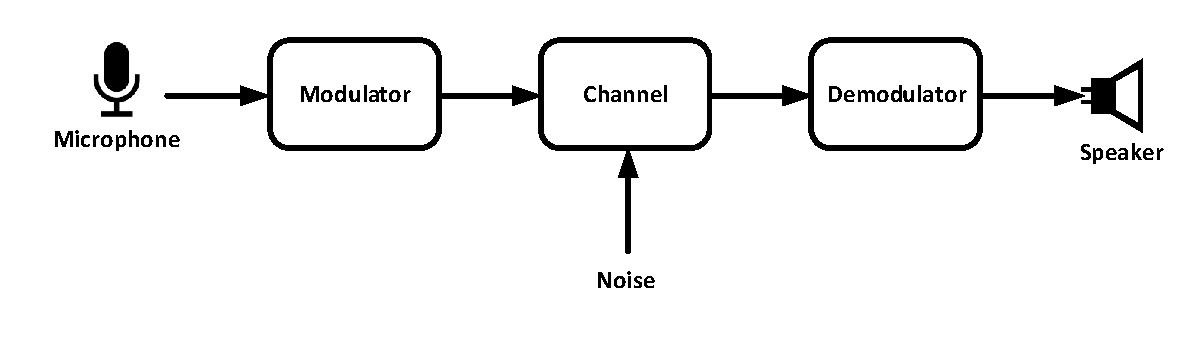
\includegraphics[scale=0.8]{Fig/model.pdf}
\caption{Block diagram of an analog communication system.}\label{fig:model}
\end{figure}

%--------------------------------------------
$$$$
\section*{Note}
At first I wrote the code for part a, b and d for continous form. But because voice is discrete I should've used digital to analog converter which is toooooooo slow. So I wrote another code which is discrete so there is no need for digital to analog converter. But for part a, b and d method 1 is okay. So for these parts I uploaded both methods. \\
In part a, b and d by "method 1" I mean the continuous method and by "method 2" I mean the discrete method.
$$$$
\section*{How to run the code}
Running the codes for method 1: \\
Please go "Codes" folder and then go to "Method 1" folder and run Main.m\\
In Main.m the results for PM and DSB after running will be plotted. But I commented the plot of SNR because it takes too much time. To test the SNR please uncomment lines 16 and 17\\
Running the codes for method 2: \\
Please go "Codes" folder and then go to "Method 2" folder. To run part e for DSB open real-time-dsb, to run part e for PM open real-time-pm and to run part a, b, c and d open main.m. Note that in main there are three sections. To test part b,d(DSB) run section 1, to test part c(DSB) run section 2, to test part a,c,d(PM) run section 3

\begin{subquestion}{Assume that the modulator and demodulator are PM. Write a MATLAB code to simulate the PM communication system. Create separate MATLAB functions for the modulator, demodulator, and channel. Then, connect them in a main mfile. Name the functions pm\_modulator, channel, and pm\_demodulator.
} 
\answer{
\lstset{language=Matlab,%
    %basicstyle=\color{red},
    breaklines=true,%
    morekeywords={matlab2tikz},
    keywordstyle=\color{blue},%
    morekeywords=[2]{1}, keywordstyle=[2]{\color{black}},
    identifierstyle=\color{black},%
    stringstyle=\color{mylilas},
    commentstyle=\color{mygreen},%
    showstringspaces=false,%without this there will be a symbol in the places where there is a space
    numbers=left,%
    numberstyle={\tiny \color{black}},% size of the numbers
    numbersep=9pt, % this defines how far the numbers are from the text
    emph=[1]{for,end,break},emphstyle=[1]\color{red}, %some words to emphasise
    %emph=[2]{word1,word2}, emphstyle=[2]{style},    
}
\section*{METHOD 1}
For PM modulation we know that 
$$u(t) = A_c cos(2 \pi f_c t + \phi(t)) = A_c cos(2 \pi f_c t + k_p m(t))$$
where $k_p$ is called phase deviation constant.
So the code for this formula will be:\\
\lstinputlisting{PM_modulator.m}
$$$$
Also for demodulation, we first calculate the derivative of the input signal, and then after finding the envelope, we calculate its integral:\\
\lstinputlisting{PM_demodulator.m}
$$$$
for channel we only add an awgn noise to the input signal\\
Channel: \\
\lstinputlisting{channel.m}
$$$$
in the following code, we have defined a function named "PM-System" which uses the above three functions and gets an input signal with modulation characteristics and gives the demodulated output and plots the results. The results are plotted in figure 2. \\
\lstinputlisting{Main_PM_part_a.m}
$$$$
\section*{METHOD 2}
This method is discrete which is faster for voice in part c and e. For PM modulation we calculate lowpass of upsampled signal and then according to the formula of PM modulatoin we calculate the modulated signal (in general for modulator we also need a bandpass filter(for fdm). But because in this project we only have one message so here we do not need a bandpass filter. But because we have noise so to find snr we need a bandpass filter in demodulator)
\lstinputlisting{pm_modulator_1.m}
Then we should pass the modulated signal through the channel. For channel we get the modulated signal, W and N0.Then using the following formulas we find the noise power and the signal power.
$$noise\;power = \frac{2N0}{2B} \;\;\;\;\; signal\;power = mean(mod.^2)$$
Then by dividing the powers we find the snr. Note that awgn function in MATLAB gets snr. So by the above formulats in our function we find the snr. \\
\lstinputlisting{channel_2.m}
$$$$
Since we have noise so to find snr we need a bandpass filter in demodulator. After the bandpass filter we use FM2AM method to find the demodulated signal. In this method we first calculate the derivative of the input, then we use an envelope detecter and after calculating the integral we remove the DC part. Figures 3 and 4 are to better illustrate these things. \\
\lstinputlisting{pm_demodulator_2.m}
}
\begin{figure}[H]
\centering
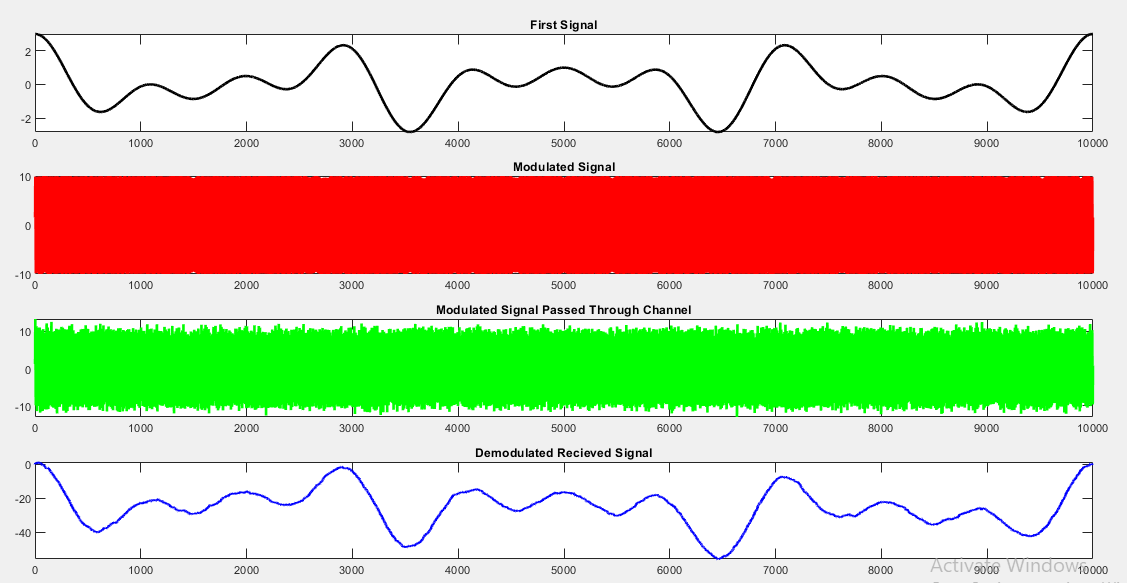
\includegraphics[scale=0.6]{Fig/2.png}
\caption{PM}\label{fig:MainPM}
\end{figure}

\begin{figure}[H]
\centering
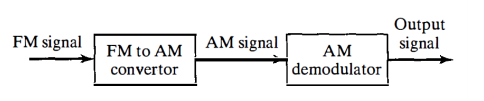
\includegraphics[scale=1]{Fig/3.png}
\caption{FM to AM demodulator with differentiator}
\end{figure}

\begin{figure}[H]
\centering
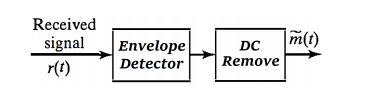
\includegraphics[scale=1]{Fig/4.png}
\caption{Block diagram of the AM envelope Demodulator}
\end{figure}

\begin{figure}[H]
\centering
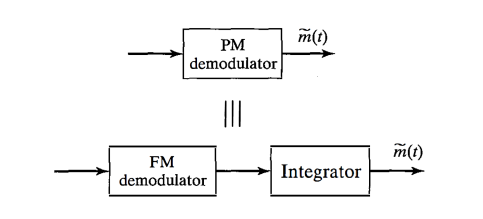
\includegraphics[scale=1]{Fig/5.png}
\caption{: A comparison of frequency and phase demodulators}
\end{figure}

\begin{figure}[H]
\centering
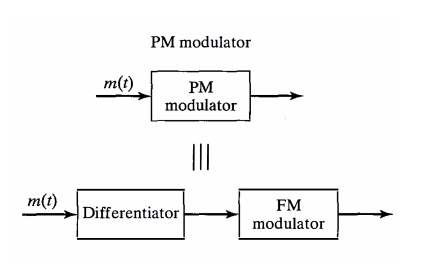
\includegraphics[scale=1]{Fig/6.png}
\caption{ A comparison of frequency and phase modulators}
\end{figure}

\end{subquestion}

%--------------------------------------------
\begin{subquestion}{Repeat the previous part for a DSB communication system. Note that the channel function does not change. You only need to code two new functions for the DSB modulator and demodulator. Name these new functions dsb\_modulator and dsb\_demodulator.}
\answer{
\lstset{language=Matlab,%
    %basicstyle=\color{red},
    breaklines=true,%
    morekeywords={matlab2tikz},
    keywordstyle=\color{blue},%
    morekeywords=[2]{1}, keywordstyle=[2]{\color{black}},
    identifierstyle=\color{black},%
    stringstyle=\color{mylilas},
    commentstyle=\color{mygreen},%
    showstringspaces=false,%without this there will be a symbol in the places where there is a space
    numbers=left,%
    numberstyle={\tiny \color{black}},% size of the numbers
    numbersep=9pt, % this defines how far the numbers are from the text
    emph=[1]{for,end,break},emphstyle=[1]\color{red}, %some words to emphasise
    %emph=[2]{word1,word2}, emphstyle=[2]{style},    
}
\section*{METHOD 1}
The formula for dsb modulation that was introduced in slides is 
$$u(t) = A_c m(t) cos( 2 \pi f_c t)$$
So like this formula, its code will be \\
\lstinputlisting{DSB_modulator.m}
$$$$
Also for demodulation we first multiply it by $cos(2 \pi f_c t)$ then we pass it through a lowpass filter. So \\
\lstinputlisting{DSB_demodulator.m}
$$$$
In Main.m we defined a function named DSB-System which gets a signal(with modulation characteristics) as an input and then by using three functions gives the demodulated output signal and plots it. The results are plotted in figure 7. \\
\lstinputlisting{Main_DSB_part_b.m}
$$$$
\section*{METHOD 2}
First we do a mixing by multiplying the message and the carrier. Then we apply a bandpass filter on modulated signal. Then we find the convolution of mixed and bandpass filter.\\
\lstinputlisting{dsb_modulator_2.m}
$$$$
Again, for demodulation we do mixing, then by applying a lowpass filter then we find the convolution pf mixed signal and lowpass filter. So we have \\
\lstinputlisting{dsb_demodulator_2.m}
$$$$
We combine these functions in main. So we have \\
\lstinputlisting{dsb_main_2.m}
}
\begin{figure}[H]
\centering
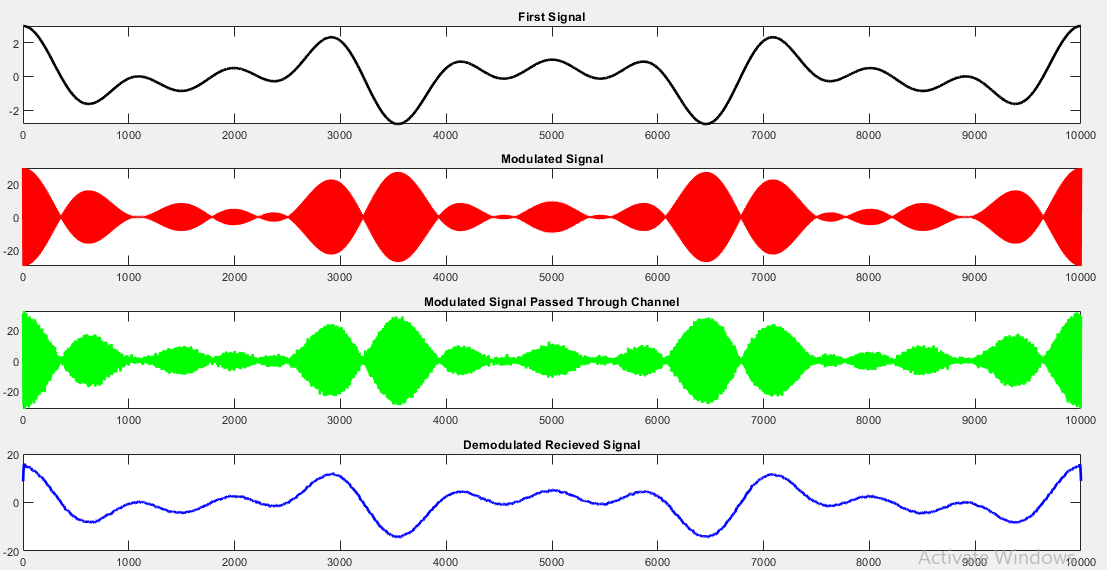
\includegraphics[scale=0.6]{Fig/7.png}
\caption{DSB}
\end{figure}
\end{subquestion}



%--------------------------------------------
\begin{subquestion}{Feed your simulation codes with a recorded audio file and play the demodulated signal and hear it for different noise levels in the channel. How do you feel when you hear the demodulated signal? Note that you can record your voice from your laptop microphone and feed it to the modulator. You can also play the demodulated signal and hear it from your laptop speaker. MATLAB has useful internal commands for working with microphones and speakers!
} 
\answer{
\lstset{language=Matlab,%
    %basicstyle=\color{red},
    breaklines=true,%
    morekeywords={matlab2tikz},
    keywordstyle=\color{blue},%
    morekeywords=[2]{1}, keywordstyle=[2]{\color{black}},
    identifierstyle=\color{black},%
    stringstyle=\color{mylilas},
    commentstyle=\color{mygreen},%
    showstringspaces=false,%without this there will be a symbol in the places where there is a space
    numbers=left,%
    numberstyle={\tiny \color{black}},% size of the numbers
    numbersep=9pt, % this defines how far the numbers are from the text
    emph=[1]{for,end,break},emphstyle=[1]\color{red}, %some words to emphasise
    %emph=[2]{word1,word2}, emphstyle=[2]{style},    
}
For audio we have two options. First option is recording our voice and after a few seconds play it. The second option is using a recorded audio. To explain both options for PM we used option 1 and for DSB we used option 2.\\
The code for PM using option 1(voice) is \\
\lstinputlisting{voice_PM.m}
$$$$
As we increase the noise of the channel or the bandwidth of the channel, our voice becomes more noisy and finally our voice is not understandable at all.
$$$$
The code for DSB using option 2(audio) is \\
\lstinputlisting{audio_DSB.m}
$$$$
As we increase the noise of the channel or the bandwidth of the channel, the audio becomes more noisy and finally it is not understandable at all.
}
\end{subquestion}

%--------------------------------------------
\begin{subquestion}{Compare the SNR performance of the simulated PM and DSB communication systems. To do this, you can plot the output SNR of both systems in terms of the channel noise level, message bandwidth, and so on.
}
\answer{
\lstset{language=Matlab,%
    %basicstyle=\color{red},
    breaklines=true,%
    morekeywords={matlab2tikz},
    keywordstyle=\color{blue},%
    morekeywords=[2]{1}, keywordstyle=[2]{\color{black}},
    identifierstyle=\color{black},%
    stringstyle=\color{mylilas},
    commentstyle=\color{mygreen},%
    showstringspaces=false,%without this there will be a symbol in the places where there is a space
    numbers=left,%
    numberstyle={\tiny \color{black}},% size of the numbers
    numbersep=9pt, % this defines how far the numbers are from the text
    emph=[1]{for,end,break},emphstyle=[1]\color{red}, %some words to emphasise
    %emph=[2]{word1,word2}, emphstyle=[2]{style},    
}
\section*{METHOD 1}
To find the SNR in output, first we pass noise from the modulator, channel and demodulator, and then we pass the signal. The output signal is a noisy signal. So if we remove the noise we get the signal. So now we have the signal and noise so by "cumsum" we can find the power of noise and signal and by dividing them, we get the snr. We plot the snr with respect to different snrs of the channel. The plot is in figure 8.\\
As we can see from the figure 8: 1)the snr of PM is bigger than the snr of DSB,
\;\;\;\;\;\;\;\;\;\;\;\;\;\;\;\; 2)if we increase the snr of the channel(or equivalently decrease the bandwidth) the snr of DSB and PM increases.(it is true that PM is a little random but by average it increases)
\lstinputlisting{snr_pm_dsb_1.m}

\section*{METHOD 2}
My PM code doesn't work properly but the logic behind the code is true. We first pass the signal through the ideal channel and we get the modulated signal and we find the power of the modulated signal. Then again we pass the same signal through the noisy channel. We get the noisy demodulated signal and if we remove the modulated signal from it, we get the noise. We find the power of the noise. By dividing the power of the demodulated signal by the power of noise we can find the snr. By doing this in a for loop for different values of bandwidth we find snr for each bandwidth. The code for this algorithm for PM is as follows \\
\lstinputlisting{pm_snr_2.m}
$$$$
For calculating the SNR of DSB, we first pass the signal through the ideal channel and we get the modulated signal and we find the power of the modulated signal. Then again we pass the same signal through the noisy channel. We get the noisy demodulated signal and if we remove the modulated signal from it, we get the noise. We find the power of the noise. By dividing the power of the demodulated signal by the power of noise we can find the snr. By doing this in a for loop for different values of bandwidth we find snr for each bandwidth. The code for this algorithm for DSB is as follows \\
\lstinputlisting{dsb_snr_2.m}
$$$$
The results for DSB is in figure 9\\
As we can see from the figure 9, if the bandwidth increases, the SNR decreases(as we expected from what we learned in the course)
}
\begin{figure}[H]
\centering
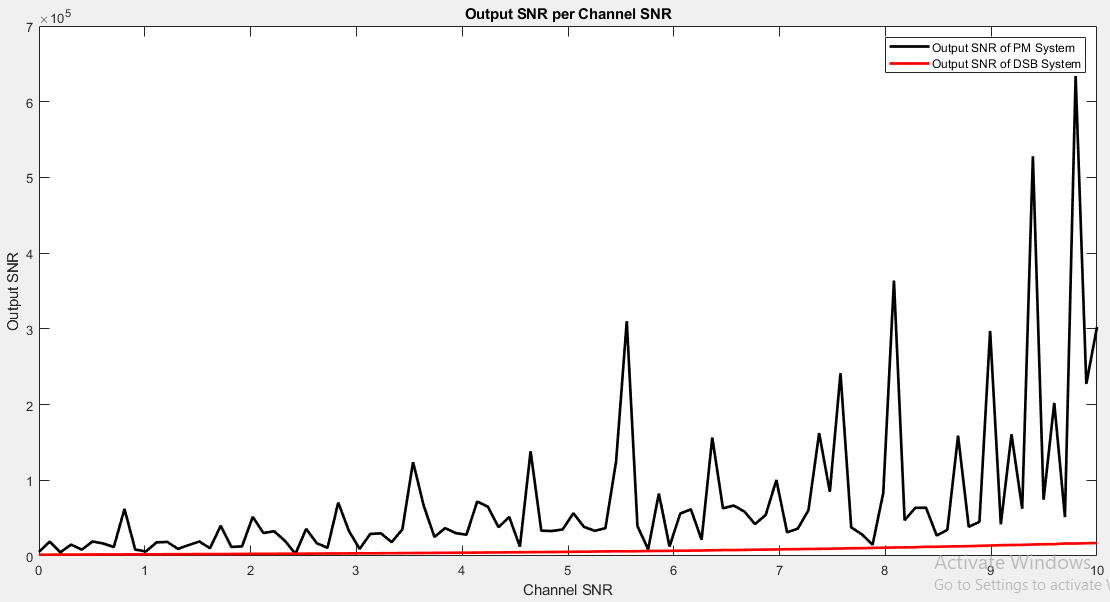
\includegraphics[scale=0.6]{Fig/9.png}
\caption{Output SNR(of DSB and PM) with respect to Channel SNR}
\end{figure}

\begin{figure}[H]
\centering
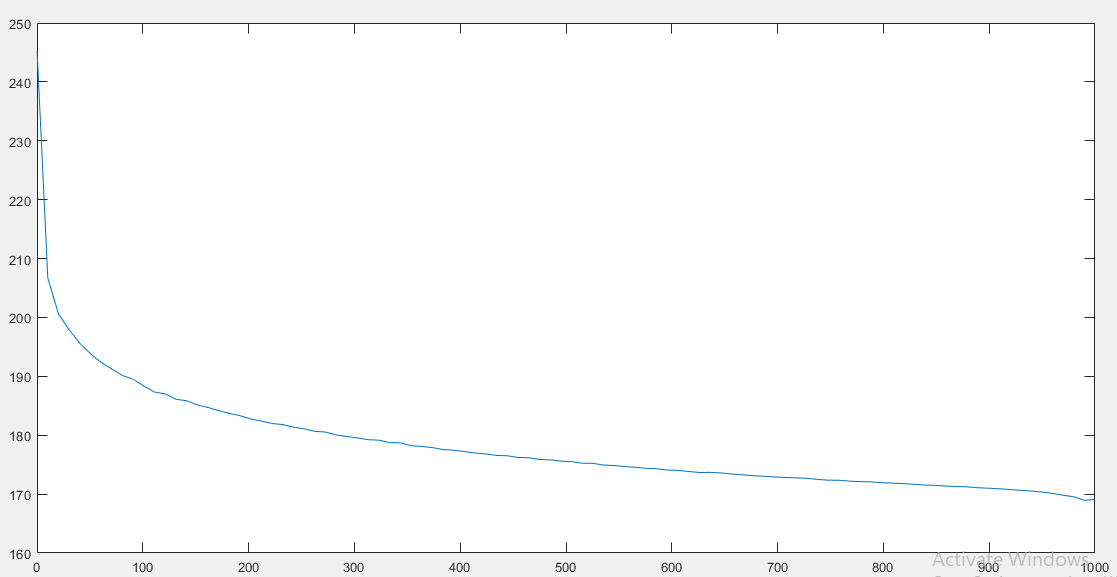
\includegraphics[scale=0.6]{Fig/8.png}
\caption{SNR of DSB with respect to the bandwidth}
\end{figure}
\end{subquestion}

%--------------------------------------------
\begin{subquestion}{Make your simulation setup realtime. In this way, you talk to the microphone and hear the demodulated signal from the speaker simultaneously without any delay and lag. 
} 
\answer{
\lstset{language=Matlab,%
    %basicstyle=\color{red},
    breaklines=true,%
    morekeywords={matlab2tikz},
    keywordstyle=\color{blue},%
    morekeywords=[2]{1}, keywordstyle=[2]{\color{black}},
    identifierstyle=\color{black},%
    stringstyle=\color{mylilas},
    commentstyle=\color{mygreen},%
    showstringspaces=false,%without this there will be a symbol in the places where there is a space
    numbers=left,%
    numberstyle={\tiny \color{black}},% size of the numbers
    numbersep=9pt, % this defines how far the numbers are from the text
    emph=[1]{for,end,break},emphstyle=[1]\color{red}, %some words to emphasise
    %emph=[2]{word1,word2}, emphstyle=[2]{style},    
}
We use an infinite loop and inside it, we get the input and then by using modulator, channel and demodulator function that we developed in part a and b, we can hear the demodulated signal\\
For DSB we have\\
\lstinputlisting{real_time_dsb.m}
$$$$
And for PM we have \\
\lstinputlisting{real_time_pm.m}
}
\end{subquestion}

%--------------------------------------------
\begin{subquestion}{Prepare a short report and describe your work concisely. Use suitable figures to better describe the developed codes and to make your report more readable and understandable. Attach a sample of the recorded audios as well as the developed codes to your sent report. 
}
\end{subquestion}

%--------------------------------------------
\begin{subquestion}{\textbf{Bonus!} Write your report in \LaTeX.
} 
\end{subquestion}
\end{question}

\end{document}
